\chapter{Cronograma}


\begin{figure}[ht]
    \begin{center}
    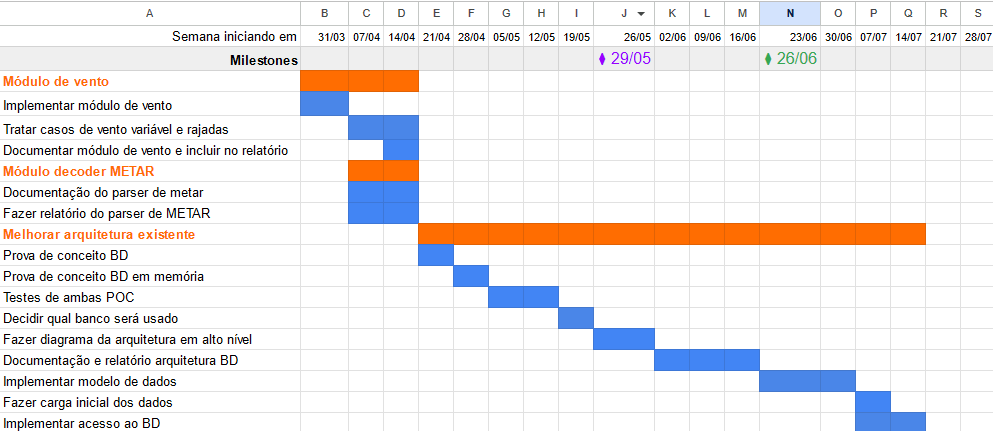
\includegraphics[width=400pt]{img/cronograma.png}
    \caption{Cronograma planejado}
    \label{fig:cronograma-planejado}
    \end{center}
\end{figure}

\begin{figure}[ht]
    \begin{center}
    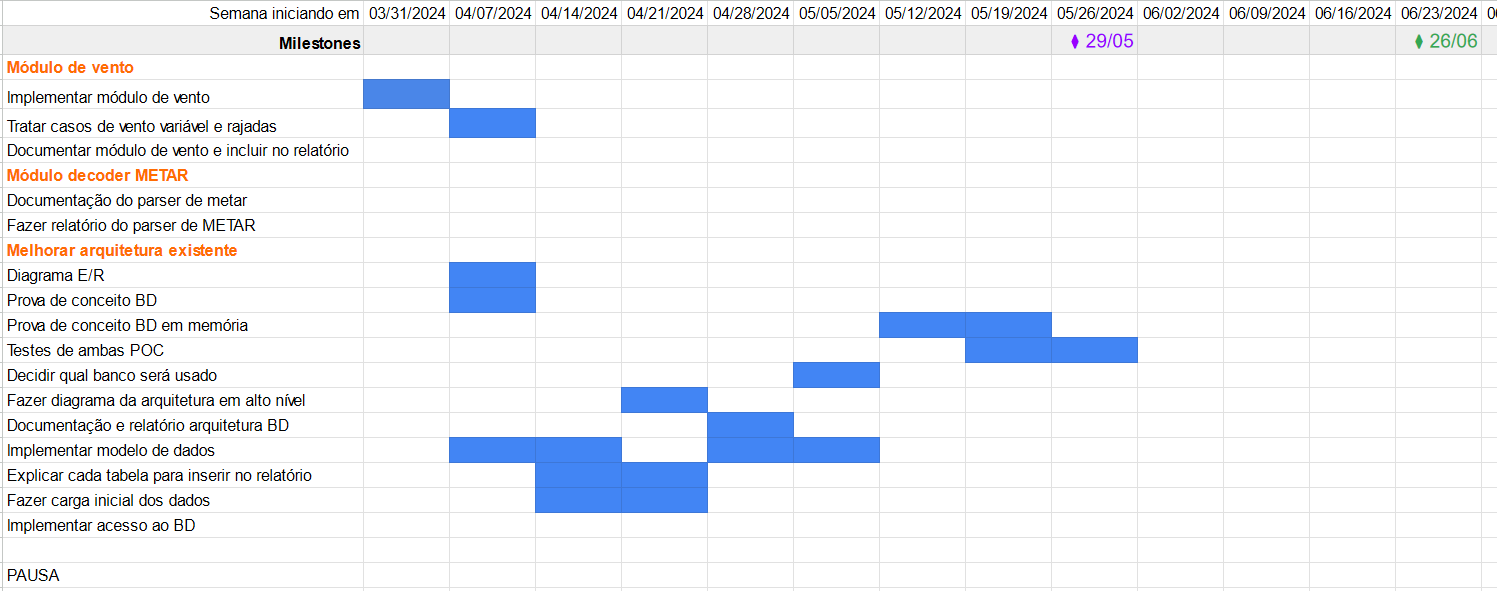
\includegraphics[width=400pt]{img/realizado.png}
    \caption{Cronograma realizado}
    \label{fig:cronograma-realizado}
    \end{center}
\end{figure}

Por ter sido meu primeiro grande projeto autogerido, tive um pouco de dificuldade em 
estimar o tempo real de implementação de cada tarefa. Portanto, há uma grande diferença entre o 
gráfico de tempo planejado e realizado.

\begin{table}[h]
    \centering
    \caption{Milestones}
    \begin{tabular}{|c|l|}
        \hline
        \textbf{Data} & \textbf{Milestone} \\
        \hline
        29/05 & Entrega da proposta de Projeto Final I \\
        26/06 & Entrega do relatório de Projeto Final I \\
        \hline
    \end{tabular}
\end{table}

